\documentclass{article}
\usepackage{tikz}
\usetikzlibrary{arrows.meta, positioning, calc, decorations.pathreplacing, decorations.markings}

\begin{document}

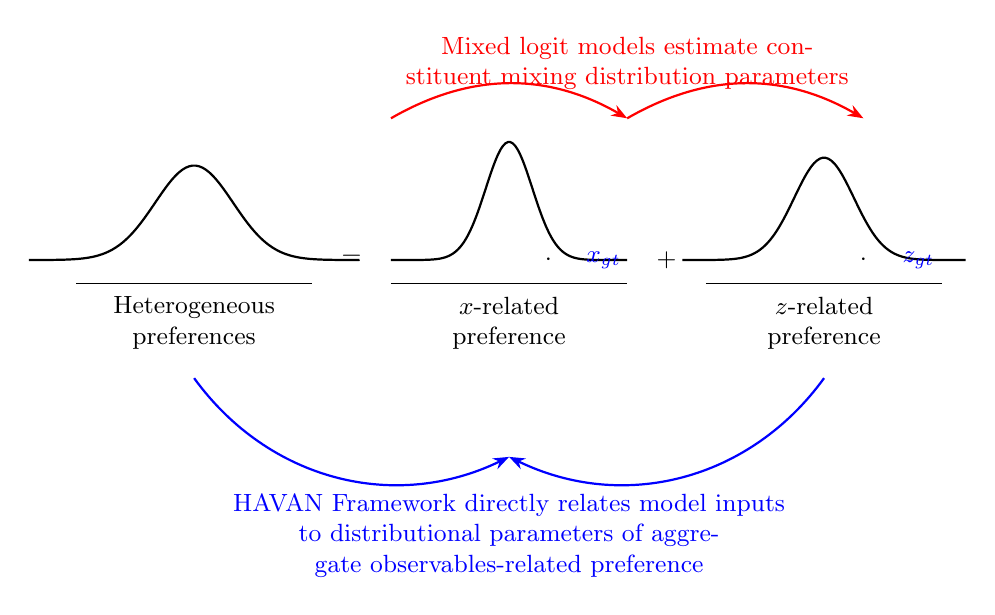
\begin{tikzpicture}[
    bell curve/.style={thick, smooth, samples=100, domain=-3:3},
    font=\small
]

% Define positions
\coordinate (left) at (0,0);
\coordinate (middle1) at (4,0);
\coordinate (middle2) at (8,0);
\coordinate (plus) at (6,0);

% Draw the bell curves
\draw[bell curve] (left) plot (\x*0.7+0, {1.2*exp(-(\x)^2/1)});
\draw[bell curve] (middle1) plot (\x*0.5+4, {1.5*exp(-(\x)^2/0.7)});
\draw[bell curve] (middle2) plot (\x*0.6+8, {1.3*exp(-(\x)^2/0.8)});

% Draw the horizontal lines
\draw (-1.5,-0.3) -- (1.5,-0.3);
\draw (2.5,-0.3) -- (5.5,-0.3);
\draw (6.5,-0.3) -- (9.5,-0.3);

% Add the "=" and "+" symbols
\node at (2,0) {$=$};
\node at (plus) {$+$};

% Add the dot symbols for weights
\node at ($(middle1) + (0.5,0)$) {$\cdot$};
\node at ($(middle2) + (0.5,0)$) {$\cdot$};

% Add the variable labels
\node[blue] at ($(middle1) + (1.2,0)$) {$x_{gt}$};
\node[blue] at ($(middle2) + (1.2,0)$) {$z_{gt}$};

% Add the labels below the curves
\node[text width=2.5cm, align=center] at (0,-0.8) {Heterogeneous preferences};
\node[text width=2.5cm, align=center] at (4,-0.8) {$x$-related preference};
\node[text width=2.5cm, align=center] at (8,-0.8) {$z$-related preference};

% Add the curved arrows and explanatory text
\draw[-{Stealth[length=2mm]}, red, thick, bend left=30] (2.5,1.8) to (5.5,1.8);
\draw[-{Stealth[length=2mm]}, red, thick, bend left=30] (5.5,1.8) to (8.5,1.8);
\node[red, text width=6cm, align=center] at (5.5,2.5) {Mixed logit models estimate constituent mixing distribution parameters};

% Add the bottom curved arrow and explanatory text
\draw[-{Stealth[length=2mm]}, blue, thick] (0,-1.5) to[bend right=40] (4,-2.5);
\draw[-{Stealth[length=2mm]}, blue, thick] (8,-1.5) to[bend left=40] (4,-2.5);
\node[blue, text width=10cm, align=center] at (4,-3.5) {HAVAN Framework directly relates model inputs\\to distributional parameters of aggregate observables-related preference};

\end{tikzpicture}

\end{document}